% 2017-03-10 - Emerson Ribeiro de Mello - mello@ifsc.edu.br
% 2023-26-09 - Paulo Fylippe Sell - paulo.sell@edu.univali.br
% \documentclass[handout,xcolor=pdftex,dvipsnames,table]{beamer}
\documentclass{beamer}

% usando tema UNIVALI-Leve
\usepackage{beamerthemeUNIVALI-LEVE}


\usepackage[utf8]{inputenc}
\usepackage[T1]{fontenc}
\usepackage[english,brazil]{babel}

% Novos tipos de colunas em tabelas que permita definir a largura
\newcolumntype{R}[1]{>{\RaggedLeft\arraybackslash}p{#1}}
\newcolumntype{C}[1]{>{\centering\arraybackslash}p{#1}}
\newcolumntype{L}[1]{>{\RaggedRight\arraybackslash}p{#1}}
\usepackage{graphicx}
\usepackage{xcolor}
\usepackage{colortbl}


% -------------------------------------------------%
% Configurações para o PDF que será gerado
% -------------------------------------------------%
\hypersetup{
    colorlinks,
    pdffitwindow=false,  % window fit to page when opened
    pdfstartview={FitH}, % fits the width of the page to the window
    linkcolor=black,  %%% cor do tableofcontents, \ref, \footnote, etc
	citecolor=black,  %%% cor do \cite
	urlcolor=black   %%% cor do \url e \href
}
% Use esse comando para fazer links para sites.
% Os links ficarão em azual e dentro dos símbolos < e > 
\newcommand{\MYhref}[3][blue]{\href{#2}{\color{#1}{<#3>}}}%
% -------------------------------------------------%


% -------------------------------------------------%
%              Título 
% -------------------------------------------------%
\title{Passeio do cavalo}
\subtitle{Implementação por meio do método de backtracking}
\author{Paulo Fylippe Sell\\Alisson Boeing}
\date{26 de setembro de 2023}
\institute{Mestrado em computação aplicada\\
	Universidade do Vale do Itajaí\\
	campus Itajaí\\
	\url{paulo.sell@edu.univali.br}\\
    \url{alisson.boeing@edu.univali.br}
}
% -------------------------------------------------%


\begin{document}

\begin{frame}[t]
    \maketitle
\end{frame}

% Descomente as linhas abaixo se desejar colocar um sumário
%\begin{frame}{Sumário}
%	\tableofcontents
%\end{frame}

%------------------------------------------------------------------------------------%
%                         Inicio do documento
%------------------------------------------------------------------------------------%

\begin{frame}{Passeio do cavalo}
    \begin{columns}
        \begin{column}{0.5\textwidth}
            \begin{itemize}
                \item Encontrar um caminho para um cavalo de xadrez em um tabuleiro;

                \item Deve visitar cada quadrado exatamente uma vez.
            \end{itemize}
        \end{column}

        \begin{column}{0.5\textwidth}
            \begin{figure}
                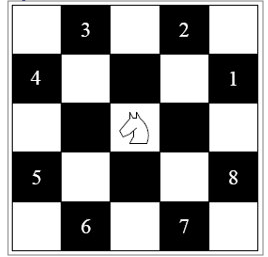
\includegraphics[scale=0.5]{figs/board.png} % Replace with your image file name and path
            \end{figure}
        \end{column}
    \end{columns}
\end{frame}


\begin{frame}{Backtracking}
    \begin{itemize}
        \item O processo de tentativa e erro constrói e percorre uma árvore de subtarefas;
        \item Passos em direção à solução final são tentados e registrados;
        \item Caso esses passos tomados não levem à solução final, eles podem ser retirados e apagados do registro.
    \end{itemize}
\end{frame}


\begin{frame}{Definição do tabuleiro}
    \includecode{python}{codigos/inicializacao.py}
\end{frame}

\begin{frame}{Inicialização do tabuleiro}
    \includecode{python}{codigos/knights_tour.py}
\end{frame}

\begin{frame}{Inicialização do tabuleiro}
    \includecode{python}{codigos/initialize_board.py}
\end{frame}

\begin{frame}{Inicialização do tabuleiro}
    \includecode{python}{codigos/knights_tour.py}
\end{frame}

\begin{frame}{Definição do caminho}
    \includecode{python}{codigos/solve_knights_tour.py}
\end{frame}

\begin{frame}{Definição do caminho}
    \includecode{python}{codigos/is_valid_move.py}
\end{frame}

\begin{frame}{Definição do caminho}
    \includecode{python}{codigos/solve_knights_tour.py}
\end{frame}

\begin{frame}{Apresentação do caminho}
    \includecode{python}{codigos/knights_tour.py}
\end{frame}

\begin{frame}{Apresentação do caminho}
    \includecode{python}{codigos/print_board.py}
\end{frame}

\begin{frame}{Apresentação do caminho}
    \includecode{python}{codigos/knights_tour.py}
\end{frame}


\begin{frame}[t]
    \maketitle
\end{frame}

\end{document}
